\documentclass[a4paper, UTF8, 12pt]{ctexart}
\usepackage{geometry}
\usepackage{listings}
\usepackage{xcolor}
\usepackage{amsmath}
\usepackage{graphicx}
\usepackage{arydshln}
\geometry{left=1.5cm, right=1.5cm, top=1.5cm, bottom=2.5cm}
\allowdisplaybreaks

\title{模式识别与机器学习作业--第四章}
\author{\ 2019.9.30}
\date{}
\begin{document}
    \maketitle
    \pagestyle{plain}
    \allowdisplaybreaks
    % \subsection*{作业1}
    \textbf{1. 设有如下三类模式样本集$w_1,w_2,w_3$,其先验概率相等,求$S_w$和$S_b$。} \newline
    \begin{equation*}
        \begin{split}
            &w_1: \ \left\{ {\left(1,0 \right)}^T, {\left(2,0\right)}^T, {\left(1,1\right)}^T \right\}, \\
            &w_2: \ \left\{ {\left(-1,0 \right)}^T, {\left(0,1\right)}^T, {\left(-1,1\right)}^T \right\}, \\
            &w_3: \ \left\{ {\left(-1,-1 \right)}^T, {\left(0,-1\right)}^T, {\left(0,-2\right)}^T \right\}, \\
        \end{split}
    \end{equation*}
    
    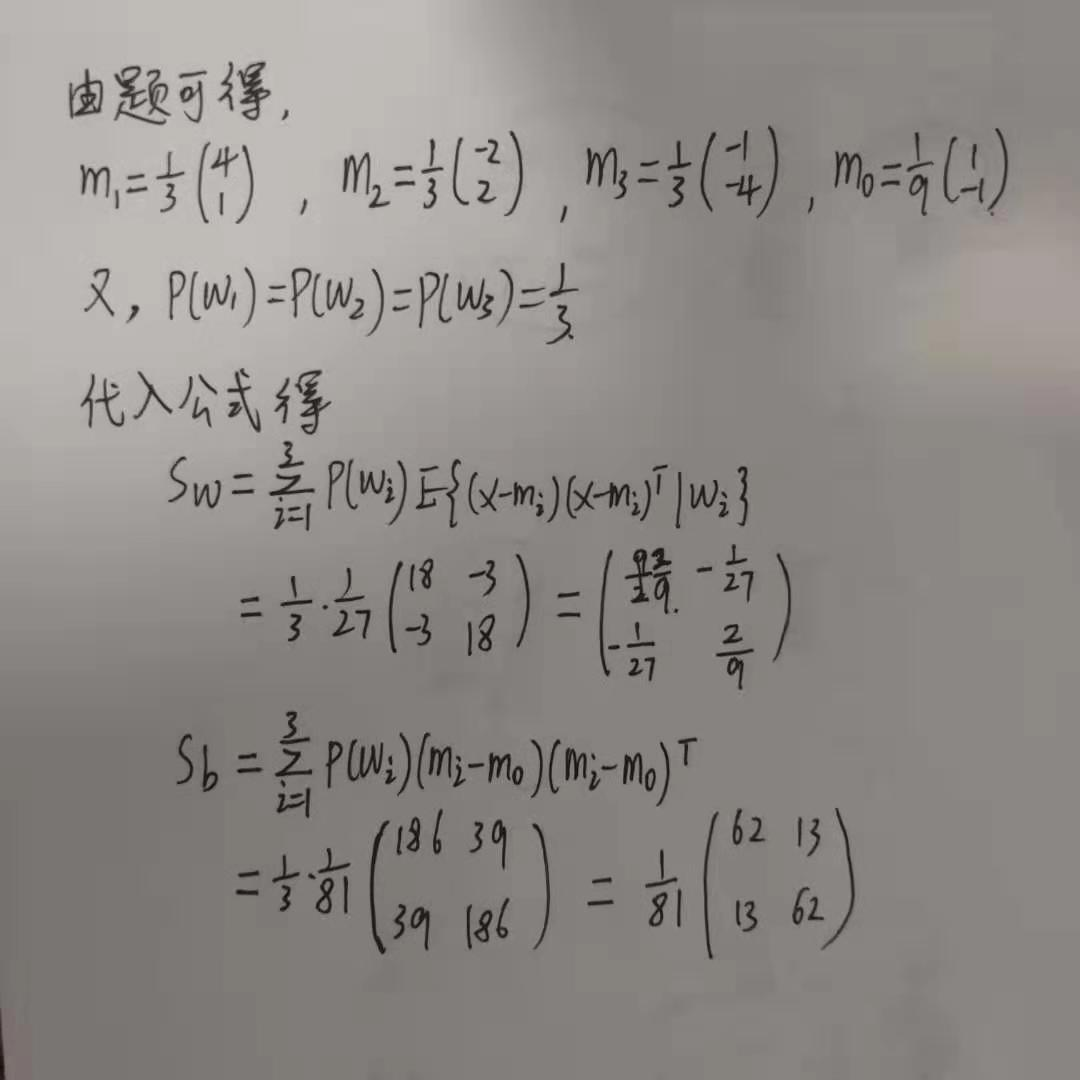
\includegraphics[scale=0.4]{asw1.jpg} \\

    % \subsection*{作业8}
    \newpage
    \textbf{2. 设有如下两类样本集,其出现的概率相等,用K-L变换,分别把特征空间维数降到二维和一维,并画出样本在该空间中的位置(可用matlab计算)。}
    \begin{equation*}
        \begin{split}
            &w_1: \ \left\{ {\left(0,0,0 \right)}^T, {\left(2,0,0 \right)}^T, {\left(2,0,1\right)}^T, {\left(1,2,0\right)}^T \right\}, \\
            &w_1: \ \left\{ {\left(0,0,1 \right)}^T, {\left(0,1,0 \right)}^T, {\left(0,-2,1\right)}^T, {\left(1,1,-2\right)}^T \right\}, \\
        \end{split}
    \end{equation*}

    由题意可以求得,样本中心点坐标为:$m=(0.75,  0.25,  0.125)^T$,由此可以求出协方差矩阵为
    \begin{equation*}
        C_x =E\left[(x-m)(x-m)^T\right] \left(
        \begin{aligned}
            &0.6875   &&0.1875  &&& -0.09375 \\
            &0.1875   && 1.1875  &&& -0.53125 \\
            &-0.09375  &&-0.53125  &&& 0.859375
        \end{aligned}\right)
    \end{equation*}
    求出其特征值和特征向量分别为:
    \begin{equation*}
        \begin{aligned}
        &\lambda_1=1.625, \  \lambda_2=0.64876246, \  \lambda_3=0.46061254 \\
        &\phi_1 =\left(
        \begin{aligned}
            0.21538745  \\
            0.95853318  \\
            -0.18660756  \\
        \end{aligned}\right), \ 
        \phi_2 =\left(
        \begin{aligned}
            0.78975397 \\
            -0.05858624  \\
            0.61061961  \\
        \end{aligned}\right), \ 
        \phi_3 =\left(
        \begin{aligned}
            -0.57436653 \\
            0.27889386 \\
            0.76962413 \\
        \end{aligned}\right)
        \end{aligned}
    \end{equation*}
    当将样本降到二维时,选择$\phi_1,\phi_2$,得
    \begin{equation*}
        \Phi =\left(
        \begin{aligned}
            &0.21538745  &&0.78975397\\
            &0.95853318  &&-0.05858624\\
            &-0.18660756  &&0.61061961 \\
        \end{aligned}\right)
    \end{equation*}
    经过线性变换后,$y=\Phi^Tx$,得
    \begin{equation*}
        \begin{aligned}
            &w_1:\left\{
                    (0. ,\    0.)^T, \ 
                    ( 0.4307  ,\   1.5795)^T, \ 
                    (0.2441  ,\  2.1901)^T, \ 
                    (2.1324 ,\   0.6725)^T
                    \right\}, \\
            &w_2:\left\{ 
                    (-0.1866 ,\   0.6106)^T, \ 
                    (0.9585  ,\ -0.0585)^T, \ 
                    (-2.1036 ,\   0.727)^T, \ 
                    (1.5471  ,\ -0.4900)^T \ 
                    \right\}
        \end{aligned}
    \end{equation*}
    降维后,样本在空间中的分布如下图所示:
    \begin{center}
        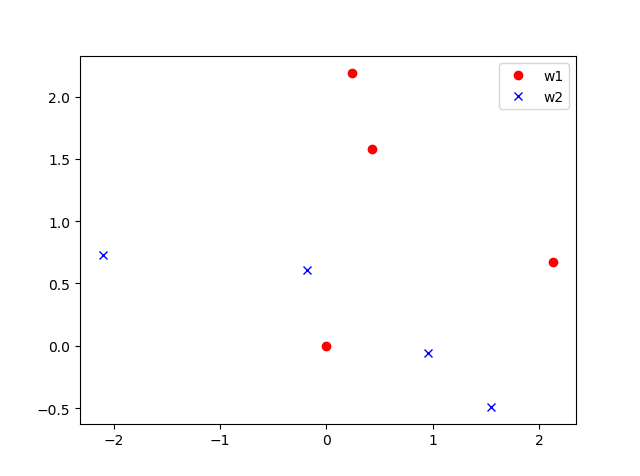
\includegraphics[scale=0.8]{asw2_1.png}
    \end{center}
    同理,当变换到一维空间中时,选择$\phi_1$进行线性变换,得
    \begin{equation*}
        \Phi =\left(
        \begin{aligned}
            &0.21538745 \\
            &0.95853318 \\
            &-0.18660756 \\
        \end{aligned}\right),\ \ \ 
        \begin{aligned}
            &w_1:\left\{
                0, 0.430,   0.2441,  2.1324
                    \right\}, \\
            &w_2:\left\{ 
                -0.1866, 0.9585, -2.1036,  1.5471
                    \right\}
        \end{aligned}
    \end{equation*}
    降维后,样本在空间中的分布如下图所示:
    \begin{center}
        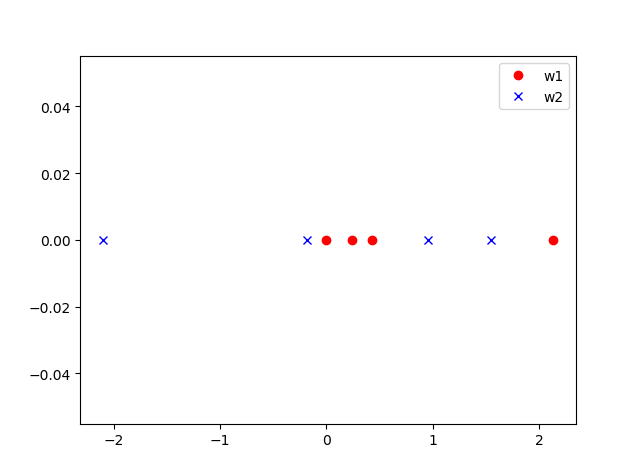
\includegraphics[scale=0.8]{asw2_2.png}
    \end{center}
\end{document}